% Nicholas M. Rathmann <rathmann@nbi.ku.dk>

\documentclass[tikz,border=0pt]{standalone}

\usepackage{pgfplots}
\usetikzlibrary{backgrounds,arrows.meta}
\usepackage{physics}
\usepackage{newtxtext,newtxmath} % RSPA-like font
\usepackage{xcolor}
\definecolor{ice}{HTML}{dcf0fd}
\definecolor{dred}{HTML}{a50f15}
\definecolor{ctheta}{HTML}{0570b0}

\tikzset{
	every picture/.style={line width=1.0pt, font=\fontsize{12}{12}\selectfont, background rectangle/.style={iceshading, shading angle=180}, show background rectangle, inner frame xsep=1ex, inner frame ysep=1ex, },	
    iceshading/.style={top color=ice!60, bottom color=gray!5},
	axis/.style={black, line width=1.0pt, -{Latex[scale=1.1]}},
	ptrarr/.style={{Stealth[scale=1.1]}-},
} 
 
\tikzset{/pgf/declare function={
	aylen = 0.6;
	axlen = 1.2;
	xr = 0.15*axlen;
	px(\z) = 0.15 + 0.2*\z + 0.1*\z^2;
	%%%
	xi = 0.35*axlen;
	dscale = 1.2;
	dz = 0.17 * aylen * dscale;
	dx = 0.26 * axlen * dscale;
}} 
 
\begin{document}
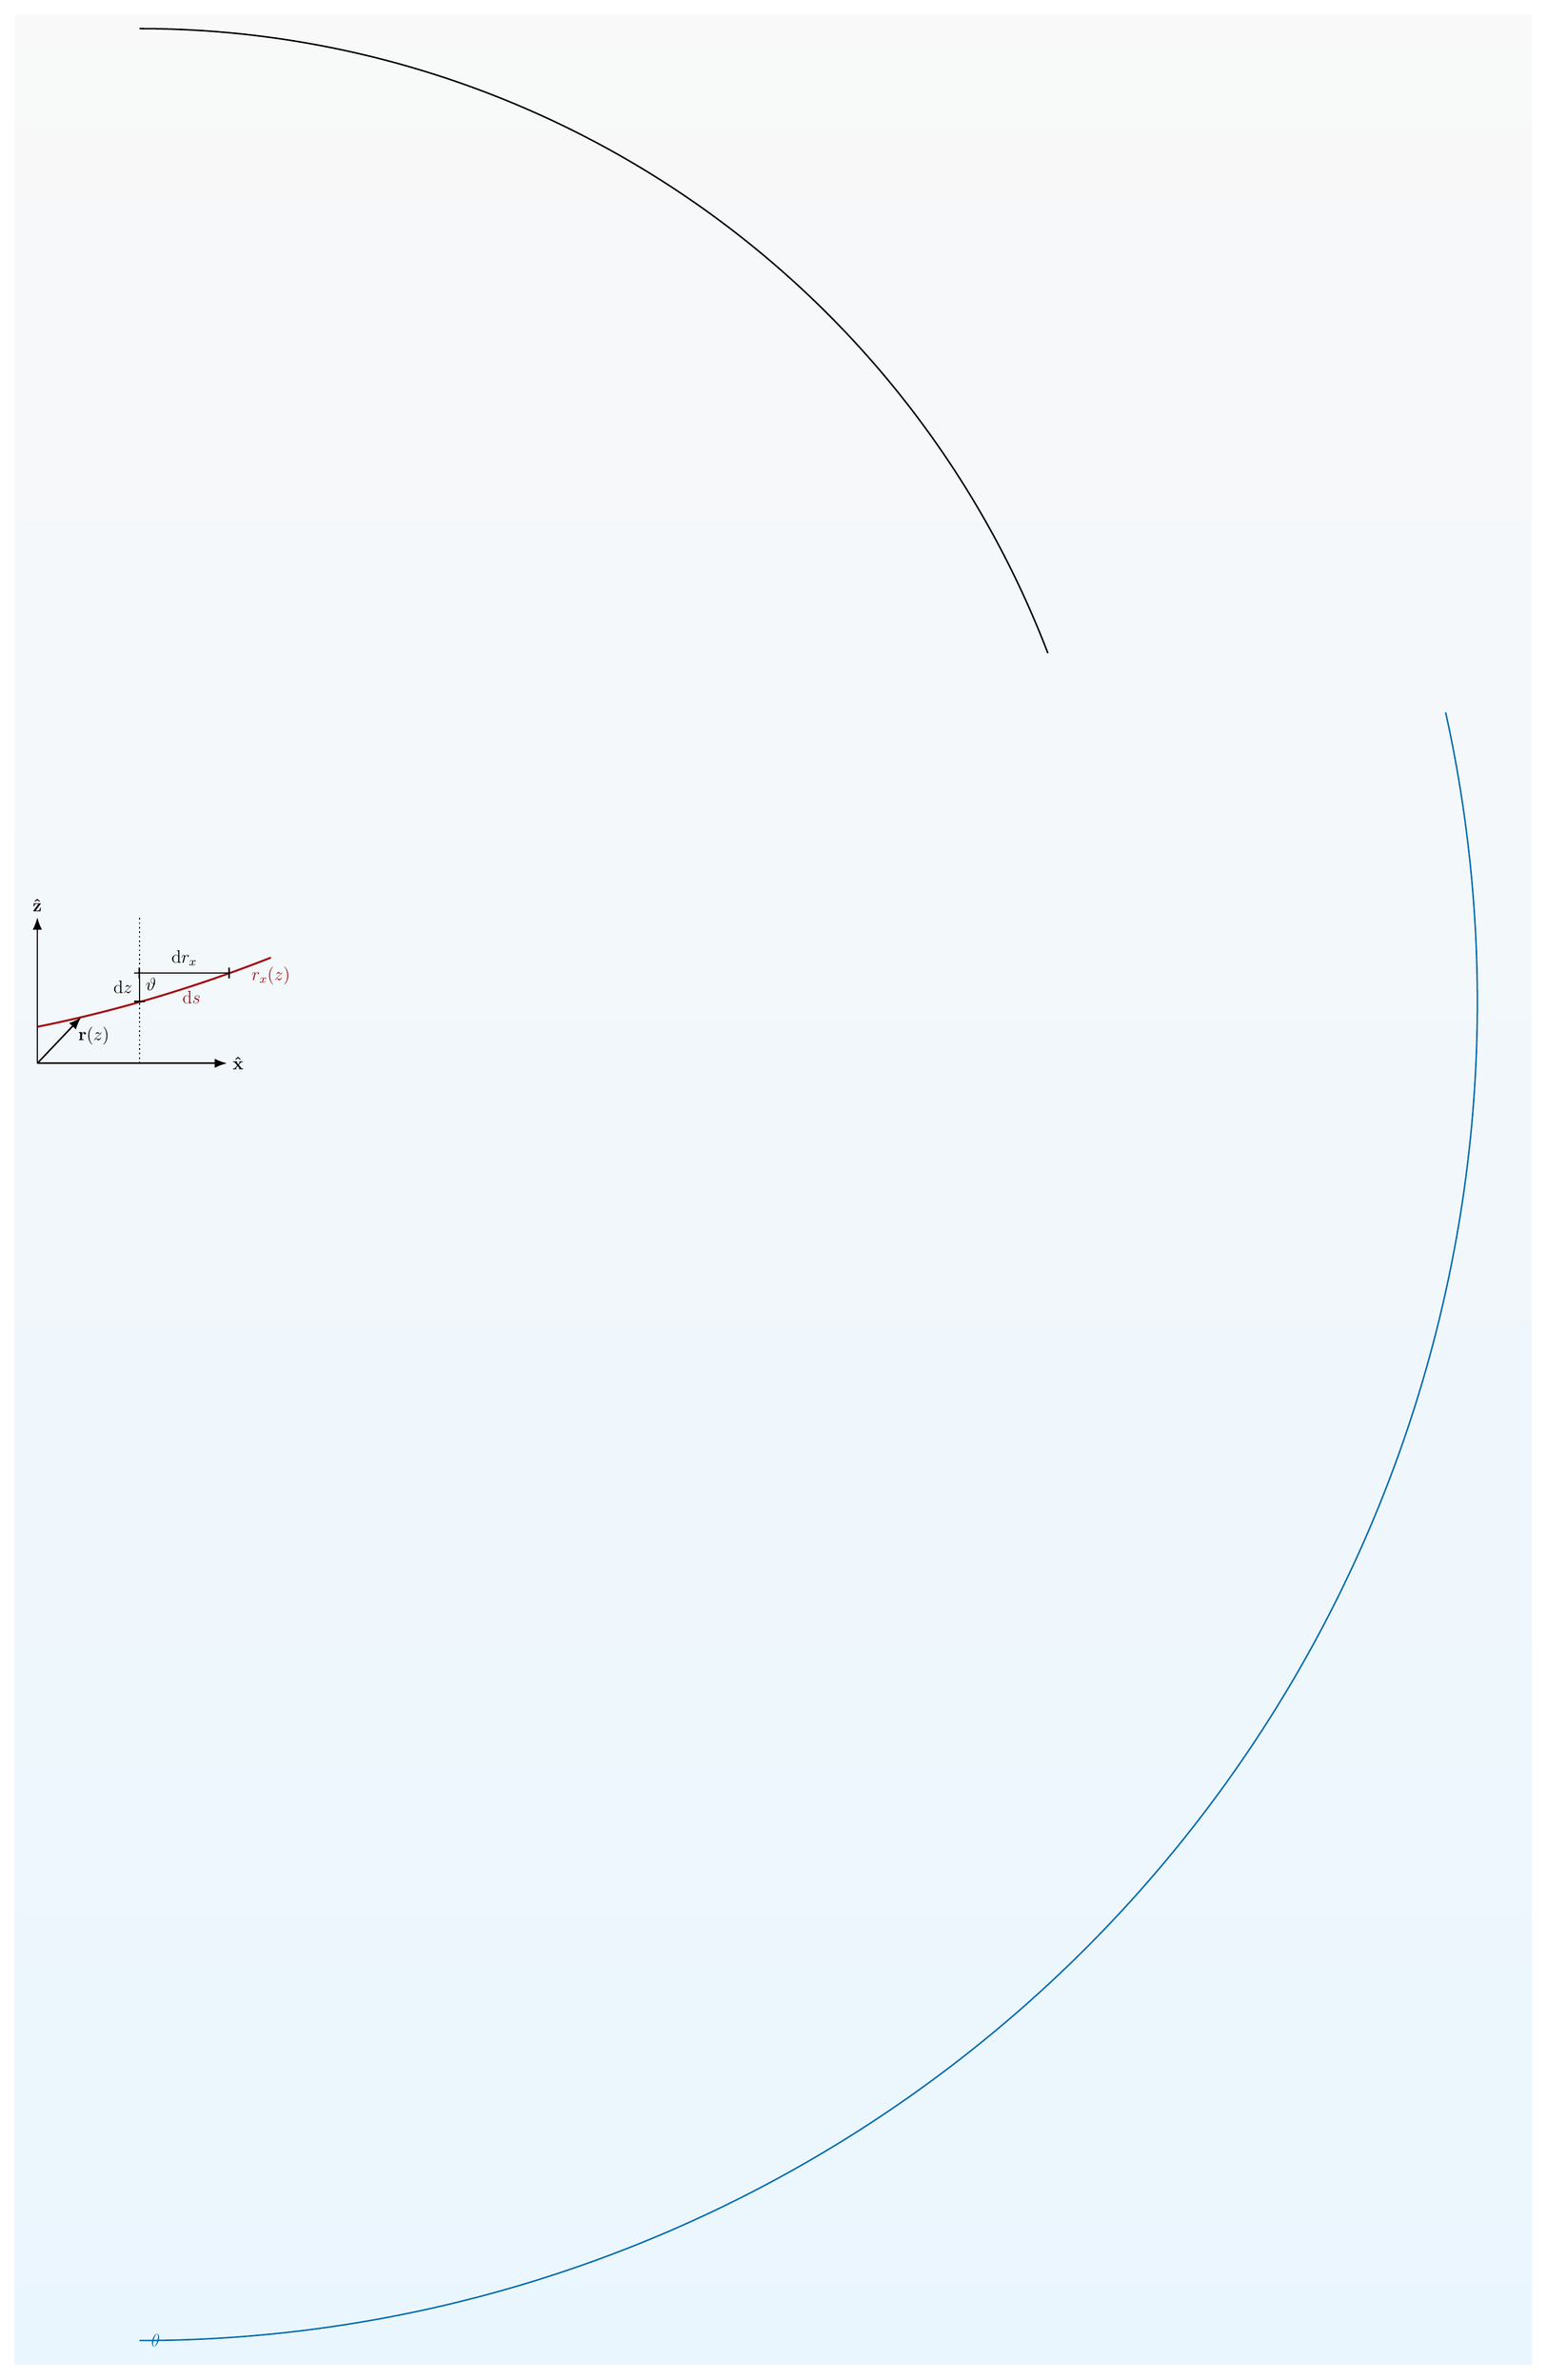
\begin{tikzpicture}[]

\begin{axis}[
        xmin=0, xmax=axlen, 
        ymin=0, ymax=aylen, 
        domain=0:{0.8*axlen}, 
        axis equal image,
		hide axis,
		clip=false,
	]
	\addplot[samples=100, dred, line width=1.3pt] {px(x)};

	\draw[axis] (axis cs:0,0) -- ++(axis cs:0,aylen) node[black,above] {$\vu{z}$};
	\draw[axis] (axis cs:0,0) -- ++(axis cs:{aylen*1.3},0) node[black,right] {$\vu{x}$};
	\draw[axis,black] (axis cs:0,0) -- (axis cs:xr,{px(xr)}) node[pos=0.6,right=0.6em] {$\vb{r}(z)$};
	\node[dred] at (axis cs:{0.8*axlen},{px(0.8*axlen)-aylen/8}) {$r_x(z)$};
	
	\draw[dotted] (axis cs:xi,0) -- ++(axis cs:0,aylen);
	
	\draw[|-|] (axis cs:{xi,px(xi)}) -- ++(axis cs:0,dz) 
		node[pos=0.5,anchor=east,left=0.1em] {$\dd{z}$}
		node[pos=0.6,anchor=west,right=+0.04em] {$\vartheta$};
		
	\draw (axis cs:{xi,px(xi)+dz}) ++(90:4) arc (90:21:4);
	
	\draw[ctheta] (axis cs:{xi,px(xi)+dz}) ++(-90:5.5) arc (-90:12.5:5.5) 
		node[pos=0.0,anchor=west,yshift=-0.0em,right=+0.4em] {$\theta$};
	
		
	\draw[|-|] (axis cs:{{xi*0.9925},{(px(xi)+dz)*0.992}}) -- ++(axis cs:dx,0) 
		node[pos=0.5,anchor=south,above=0.1em] {$\dd{r_x}$};
	
	\node[dred] at (axis cs:{xi+dx/1.75},{px(xi+dx/1.75)-aylen/13}) {$\dd{s}$};

\end{axis}	

\end{tikzpicture}
\end{document}